\documentclass{article}
\usepackage[utf8]{inputenc}
\usepackage{float}
\usepackage{graphicx}
\usepackage{gensymb}
\usepackage{animate}
\usepackage{attachfile}
\usepackage{caption}
\usepackage{subcaption}
\usepackage{pgfgantt}
\usepackage{xcolor}
\usepackage{lscape}
\usepackage{afterpage}

\title{Rover Advancements - Ceres}
\author{Nicolas Correal Murillo \and Juan Felipe Ruiz Sosa \and Jorge Montes Eljach \and Daila Natalia Mantilla Tarazona \and Diego Alejandro Prieto Fernandez \and Juanita Gallo Restrepo \and Laura Sofia Ramirez \and Juan Nicolas Gomez Jimenez \and Maria Alejandra Cardona }
\date{\today}



\begin{document}
\maketitle
\newpage

\tableofcontents

\newpage

This icon means that there is an attached file: \noattachfile{} to download it, double click it.
\section{Introduction}
We, the Ceres team, are developing a Martian exploration rover to participate in international competitions.
Our project aims to expand our knowledge in various technical fields and demonstrate the expertise we've gained
 through past robotic experiences and our professional careers. By tackling the challenges of designing and 
 building a rover capable of operating on Mars, we hope to advance our skills and contribute to the broader 
 field of space exploration. We differentiate our selves with this proyect by being the only team developing our own motors from scratch.
In this document we highlight our most relevant milestones, along with the main developments and learnings along the way, as well stating with our following steps.


\begin{landscape}
    \section{Gantt Chart - Work in Progress}
    \begin{ganttchart}[
        hgrid,
        vgrid,
        x unit=0.52cm, % Scale down horizontally
        y unit title=0.6cm, % Scale down title vertically
        y unit chart=0.5cm, % Increase vertical spacing between rows
        title/.append style={fill=yellow!80},
        title label font=\bfseries\scriptsize, % Change the size of the titles
        title label anchor/.append style={below=-1.6ex},
        title left shift=.05,
        title right shift=-.05,
        title height=.6,
        bar/.append style={fill=cyan!60},
        bar height=.5, % Adjust bar height
        bar label font=\scriptsize, % Reduce the font size of the bar labels
        bar label node/.append style={anchor=east, xshift=-0.1cm}, % Position labels to the left
        group right shift=0,
        group top shift=.6,
        group height=.3,
        group peaks tip position=0,
        milestone/.append style={fill=green!80},
        milestone height=.5, % Adjust milestone height
        milestone label font=\scriptsize, % Reduce the font size of the milestone labels
        milestone label node/.append style={anchor=east, xshift=-0.1cm} % Position milestone labels to the left
       ]{1}{28}
    
      % Title
      \gantttitle{June}{4}
      \gantttitle{July}{4}
      \gantttitle{August}{4}
      \gantttitle{September}{4}
      \gantttitle{October}{4}
      \gantttitle{November}{4}
      \gantttitle{December}{4} \\
      \gantttitlelist{1,...,28}{1} \\
    
      % Motors
      \ganttgroup{Motors}{1}{6} \\
      \ganttmilestone{1st Prototype}{1} \\
      \ganttmilestone{2nd Prototype}{2} \\
      \ganttmilestone{3rd Prototype}{3} \\
      \ganttbar{1st Internal cycloidal drive}{4}{5} \\
      \ganttbar{2nd Internal cycloidal drive}{5}{6} \\
      \ganttmilestone{Motor Characterization}{6} \\
    
      % Chasis/Rockers
      \ganttgroup{Chasis/Rockers}{2}{14} \\
      \ganttbar{First designs}{2}{14} \\
      \ganttmilestone{First Assembly - Wood}{14} \\
      \ganttmilestone{Physical Rover model}{16} \\
    
      % Wheels
      \ganttgroup{Wheels}{2}{14} \\
      \ganttbar{First designs}{2}{14} \\
      \ganttbar{First prototypes}{12}{14} \\
    
      % Arm
      \ganttmilestone{Arm Moving}{23} \\
    
      % Design and brand
      \ganttgroup{Design and brand}{11}{14} \\
      \ganttmilestone{Logo proposal}{11} \\
      \ganttbar{Animation Course}{12}{13} \\
      \ganttmilestone{Socials inauguration}{14} \\
    
      % Milestones
      \ganttmilestone{The base of the rover moves}{19} \\
      \ganttmilestone{Cameras working on rover}{20} \\
      \ganttmilestone{Rover moves with antennas}{28} \\
    
    \end{ganttchart}
    \end{landscape}


\section{Milestones Achieved}
 \subsection{Motors}

 \subsubsection{First prototype}
\paragraph{Developments}
 \begin{itemize}
    \item 100mm x 10mm Stator - 3 phase Winding
    \begin{figure}[H]
        \centering
        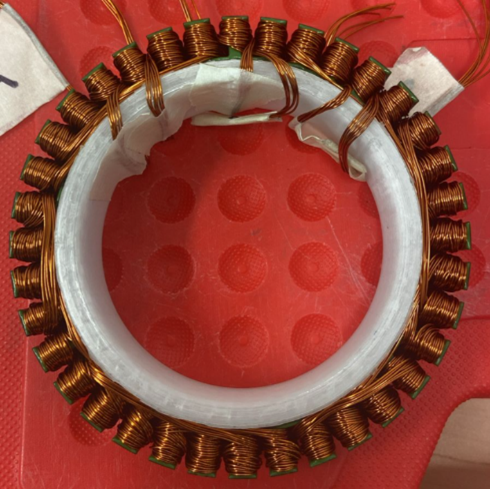
\includegraphics[width=\linewidth]{Images/Motor/Estator10010PrimerEmbobinado.png}
        \caption{First Motor Winding}
    \end{figure}
    \item 3D model of the rotor with 42 poles (magnets) along with a base
    \begin{figure}[H]
        \centering
        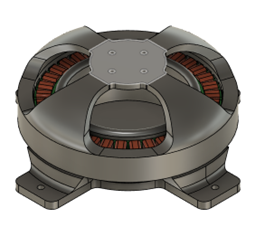
\includegraphics[width=\linewidth]{Images/Motor/PrimerPrototipo.png}
        \caption{First Prototype 3D}
    \end{figure}
    \item 3D Print of the motor and assembly
    \item Initial test with a 30A generic ESC
 \end{itemize}
\paragraph{Results}
\begin{itemize}
    \item The motor vibrates, like triying to move
    Video: \attachfile{Images/Motor/FirstTry.gif}
    \item The motor winding heats up a lot and very quickly as soon at it is turned on
    
    \begin{figure}[H]
        \centering
        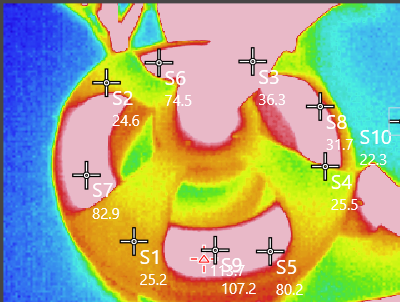
\includegraphics[width=\linewidth]{Images/Motor/MotorHeat1.png}
        \caption{Motor Heat Test}
    \end{figure}
    \item The rotor sticks to one side of the stator as it is not supported by anything at its center
    \item 2 ESC were broken due to the high current draw
\end{itemize}
\paragraph{Conclusions}
\begin{itemize}
    \item The motor base needs to have an alligment that mantains the rotor at the center of the structure
    \item An ESC with higher current capacity is needed for these tests.
    \item It is necessary to check why one of the phases was heating up to 110\degree C. As well as identifying if this was the cause of the motor not being able to spin
\end{itemize}


\subsubsection{Second prototype}
\paragraph[short]{Development}
\begin{itemize}
    \item A new motor was designed, featuring a rotor (upper part) with an extension that fit into an internal base within the stator (lower part), 
    which blocked lateral movement and limited vertical position while allowing rotational movement. Both parts were made entirely of plastic.
    \begin{figure}[H]
        \centering
        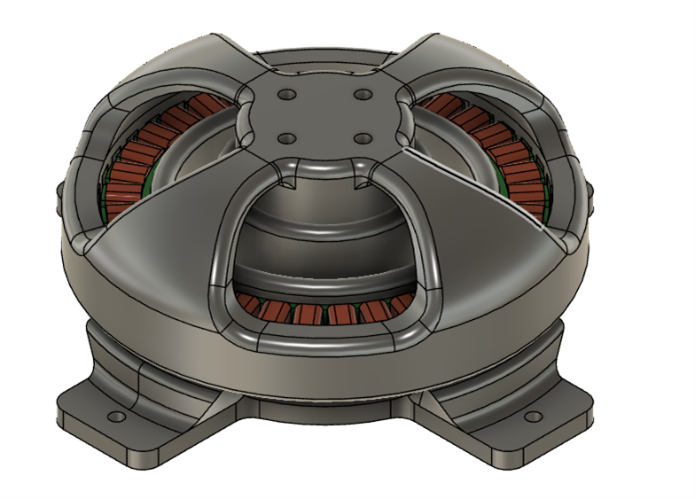
\includegraphics[width=\linewidth]{Images/Motor/SegundoPrototipo.png}
        \caption{Second Motor Prototype}
    \end{figure}
    \item The motor winding was redone because we found that some of them were wound in the opposite direction to what they should have been. 
    This caused the magnetic field, responsible for generating rotation, to be constantly canceled out.

    \item 3D printing and assembly
\end{itemize}

\paragraph{Results}
\begin{itemize}
    \item An 80A 6S ESC was used in order to use higher voltage and current when trying the motor. 
    \item The motor spins correctly, however no cuantitative methods were used to classify the success of this movement.
    \textbf{Video: \attachfile{Images/Motor/FirstSpin.gif}}

    \begin{figure}[H]
        \centering
        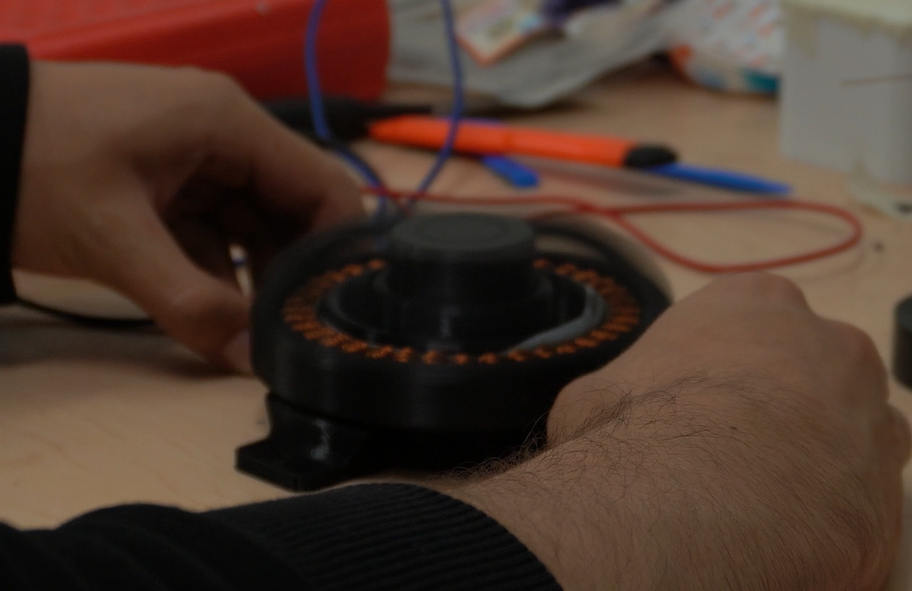
\includegraphics[width=\linewidth]{Images/Motor/FirstSpin.png}
        \caption{First Spin}
    \end{figure}
    
    \item After some time of testing, the friction between the internal support of the rotor and base of the stator make them melt together.
    \item The rotor still isnt maintained correctly in the vertical axis.
\end{itemize}
\paragraph{Conclusions}
\begin{itemize}
    \item A different alternative to maintain the rotor aligned is neccessary. One that reduces friction while maintaining the center firmly in its position.
\end{itemize}

\subsubsection{Third Protoype}


\paragraph[short]{Development}
\begin{itemize}
    \item A new 3D design of the base was created, where the connection between the base and the rotor is made using a bearing to reduce friction and improve the rigidity of the coupling between the two parts.
    \item An arm was designed for the rotor, which will help us have a basic understanding of the torque the motor can produce.
    \item The rotor design was changed so that the magnets are no longer attached with resin, allowing for faster and more efficient assembly and facilitating the effective recovery of the magnets for use in future prototypes.
    \item Printing and Assembly of the model
    \item Speed was measured with a tacometer
    \item Current was measured with a current clamp at no motor load
    \textbf{Video: \attachfile{Images/Motor/SpinCurrent.gif} (each 10mV = 1A)}
    \begin{figure}[H]
        \centering
        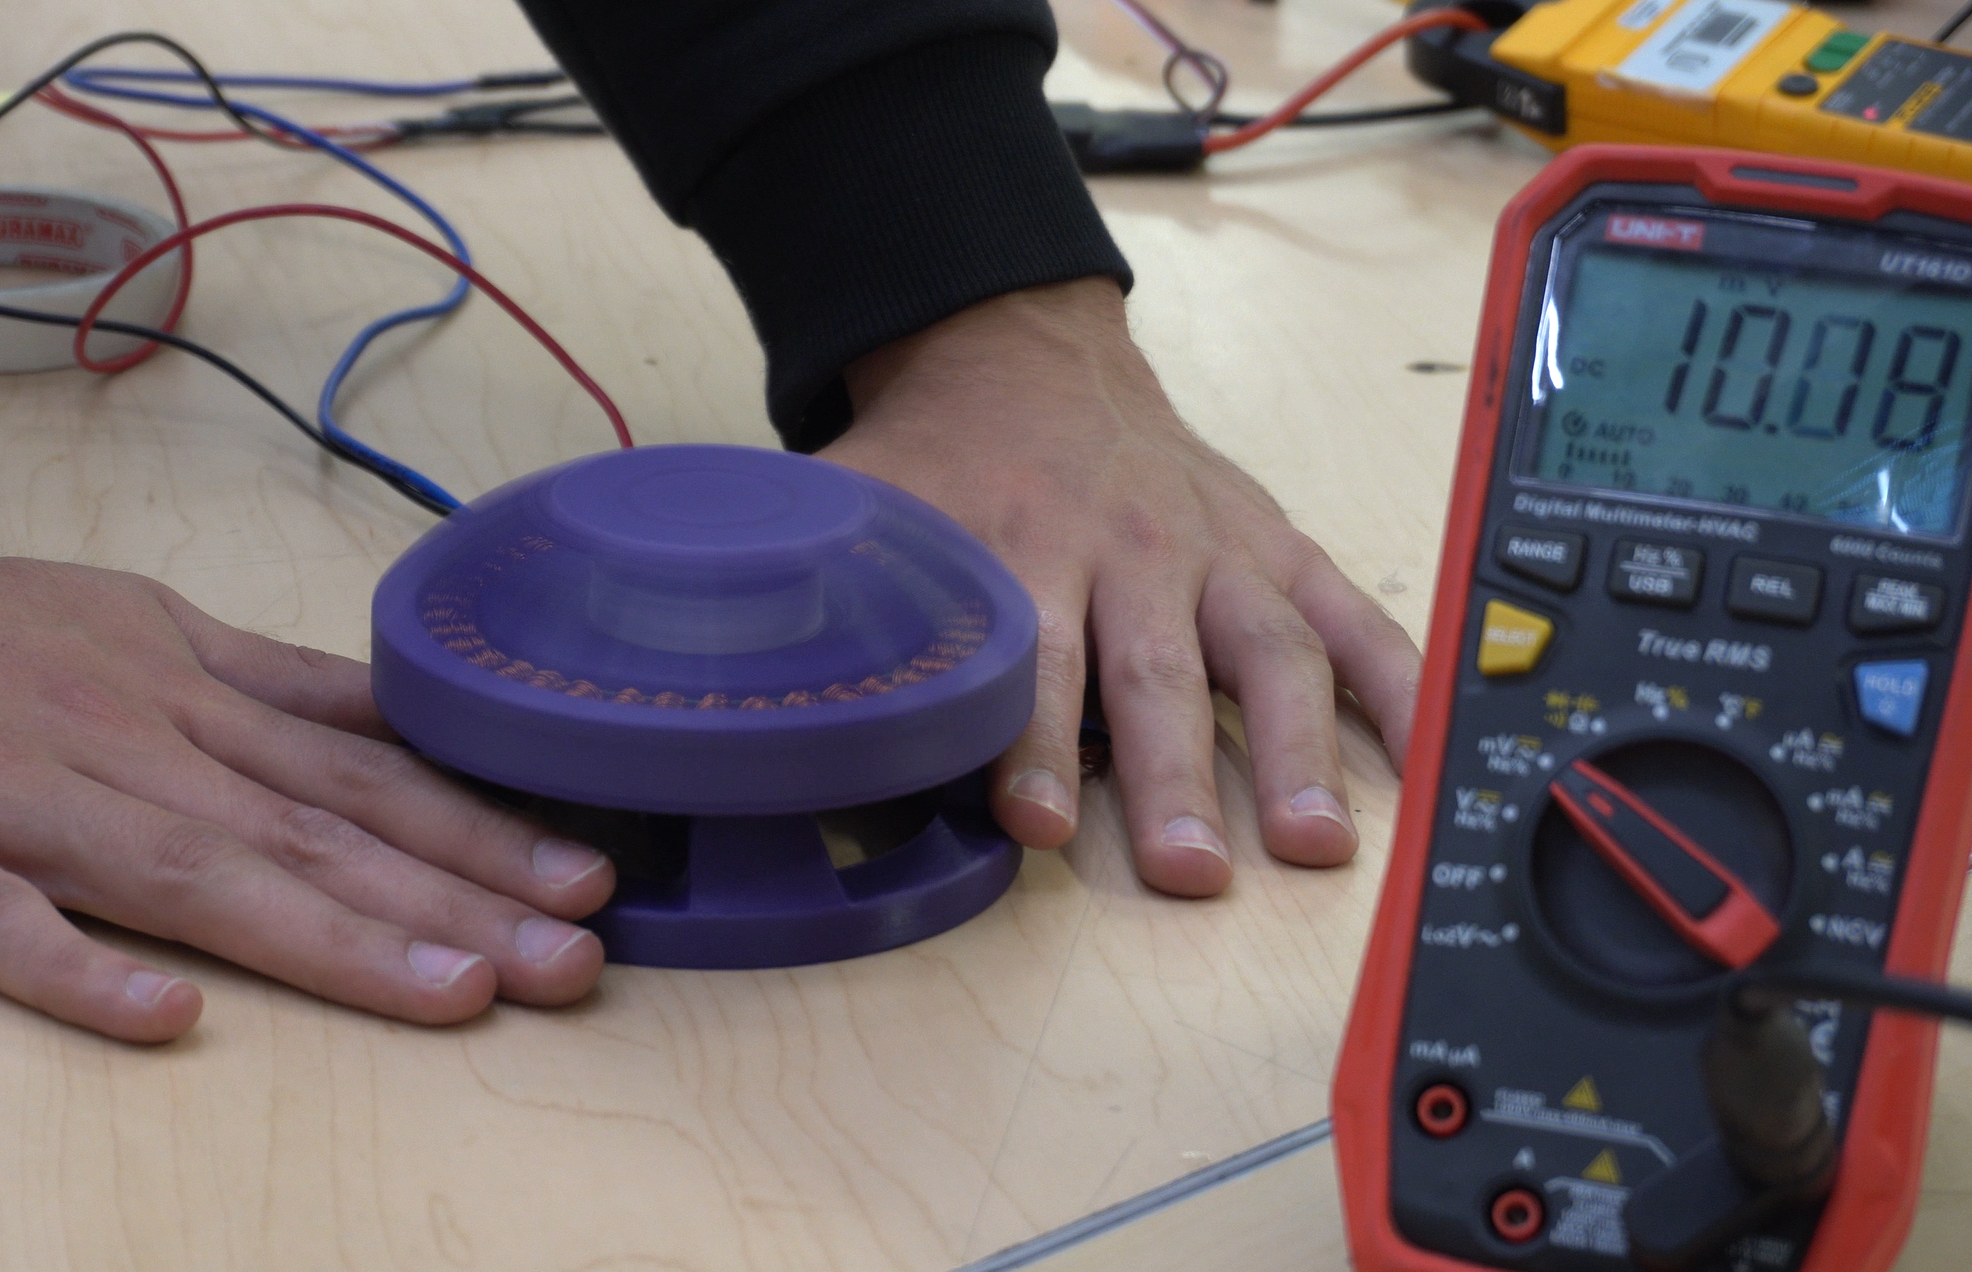
\includegraphics[width=\linewidth]{Images/Motor/CurrentMeasure.png}
        \caption{Current and Speed Measurement}
    \end{figure}
    \item Simple cualitative torque tests
\end{itemize}

\paragraph[short]{Conclusions}
\begin{itemize}
    \item The speed measured with the tacometer doesnt seem to be accurate, as it gave a far faster speed than expected (4000rpm vs 2000rpm) and after that failed to read in further tests.
    \item The motor visibly has an easier time spinnign with the bearing, as friction was greatly reduced
    \item Another way to measure the motor speed is neccessary.
    \item We need a cualitative and more safe way to measure the torque output.
\end{itemize}

\subsubsection{First Cycloidal Drive prototype}
\paragraph[short]{Development}
\begin{itemize}
    \item A cycloidal drive was designed to fit within the stator of the motor, thereby optimizing its volume. This gearbox features a central shaft which is anchored to the motor rotor. As it rotates, the discs on the shaft (highlighted in the photo) turn with the desired reduction ratio due to the shape of the ring (highlighted in the photo). To capture this reduction, the discs have holes through which the output shaft (highlighted in the photo) is inserted, rotating with the expected reduction ratio, which in this case is 8:1. Thus, for every 8 turns of the rotor, the output makes 1 turn, but with greater torque.
    \begin{figure}[H]
        \centering
        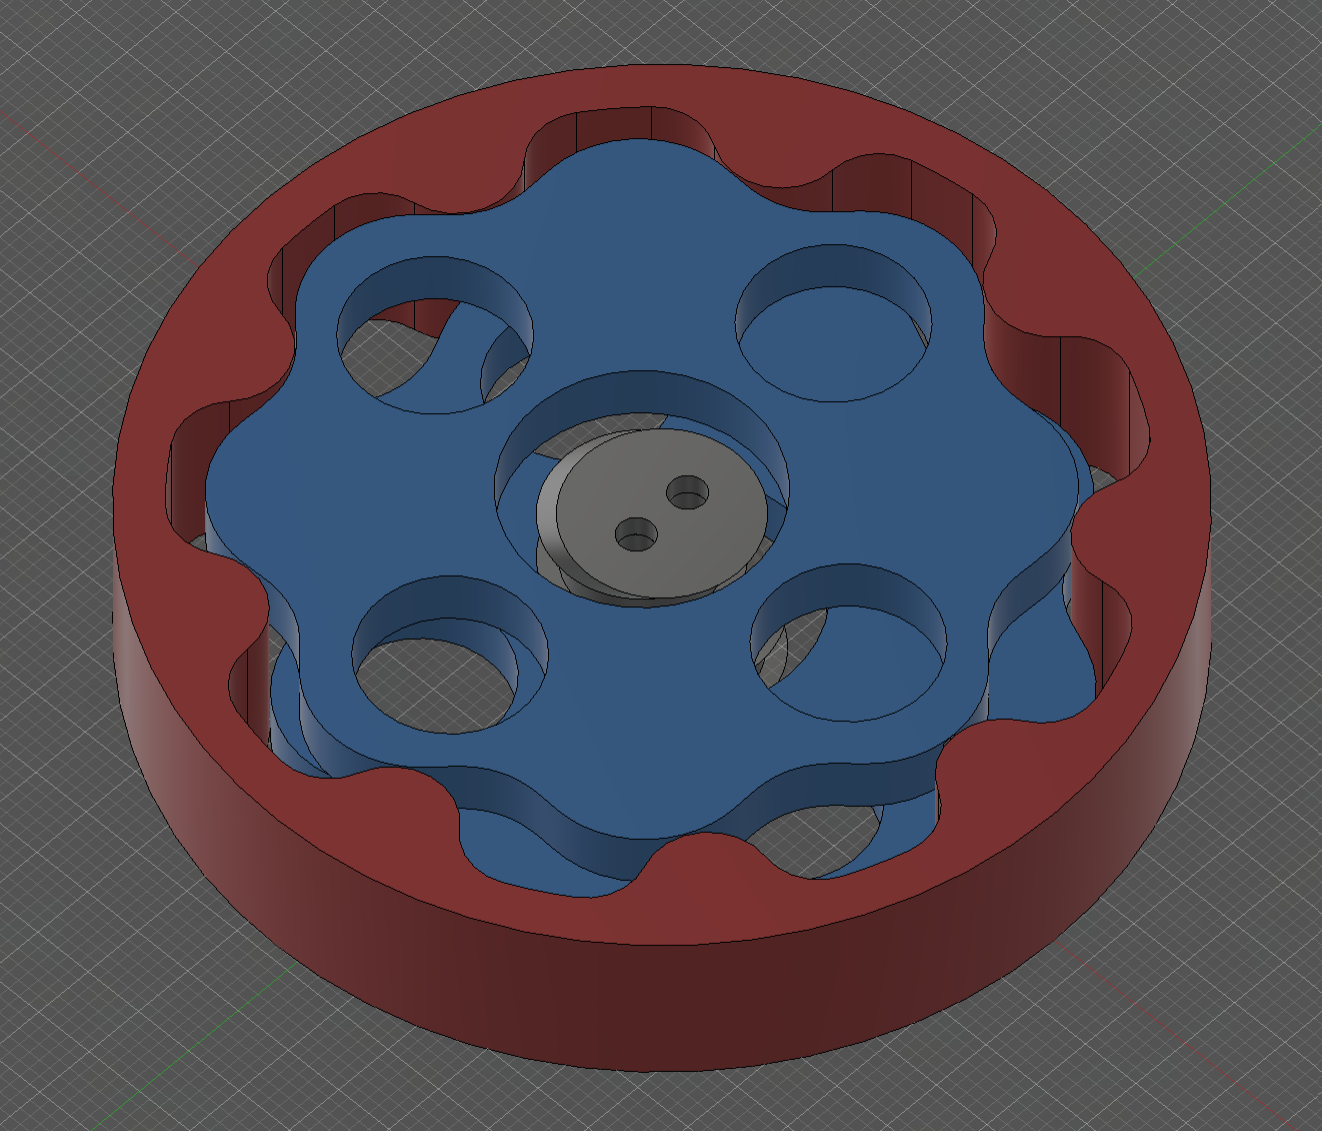
\includegraphics[width=\linewidth]{Images/Motor/CycProt.png}
        \caption{Cycloidal Drive first design}
    \end{figure}
    \item Some parts were printed to test the concept with bearings and screws, and to adjust the design based on the results.
    \item The entire prototype was 3D printed in plastic and assembled with bearings and screws.
    \item Tests were made to verify that the expected reduction in terms of rotations was being achieved.
\end{itemize}
\paragraph[short]{Results}
\begin{itemize}
    \item The cycloidal drive was operational.
    \item The expected reduction ratio of 8:1 in terms of rotations was achieved.
    \item Some screws collided due to the dimensions of the parts and the screws themselves, causing friction that hindered the gearbox's movement.
    \item The alignment method was insufficient, causing the gearbox to twist during operation.
\end{itemize}

\paragraph[short]{Conclusions}
\begin{itemize}
    \item Details such as the sizes of the parts and screws need to be adjusted so that tolerance does not interfere with the movement.
    \item The efficiency of torque transmission in the reduction needs to be calculated.
    \item With the necessary adjustments, the cycloidal drive will be ready to be assembled with the motor for testing maximum torque, speed, and consumption.
\end{itemize}

\subsubsection{First \textbf{Internal} Cycloidal Drive prototype}
\paragraph[short]{Development}
\begin{itemize}
    \item A design was created to connect the rotor (motor output) to the cycloidal drive shaft (gearbox input) located within the stator to optimize motor volume. Additionally, an external base was designed to cover the motor and support and stabilize the cycloidal drive output.
    
    \begin{figure}[H]
        \centering
        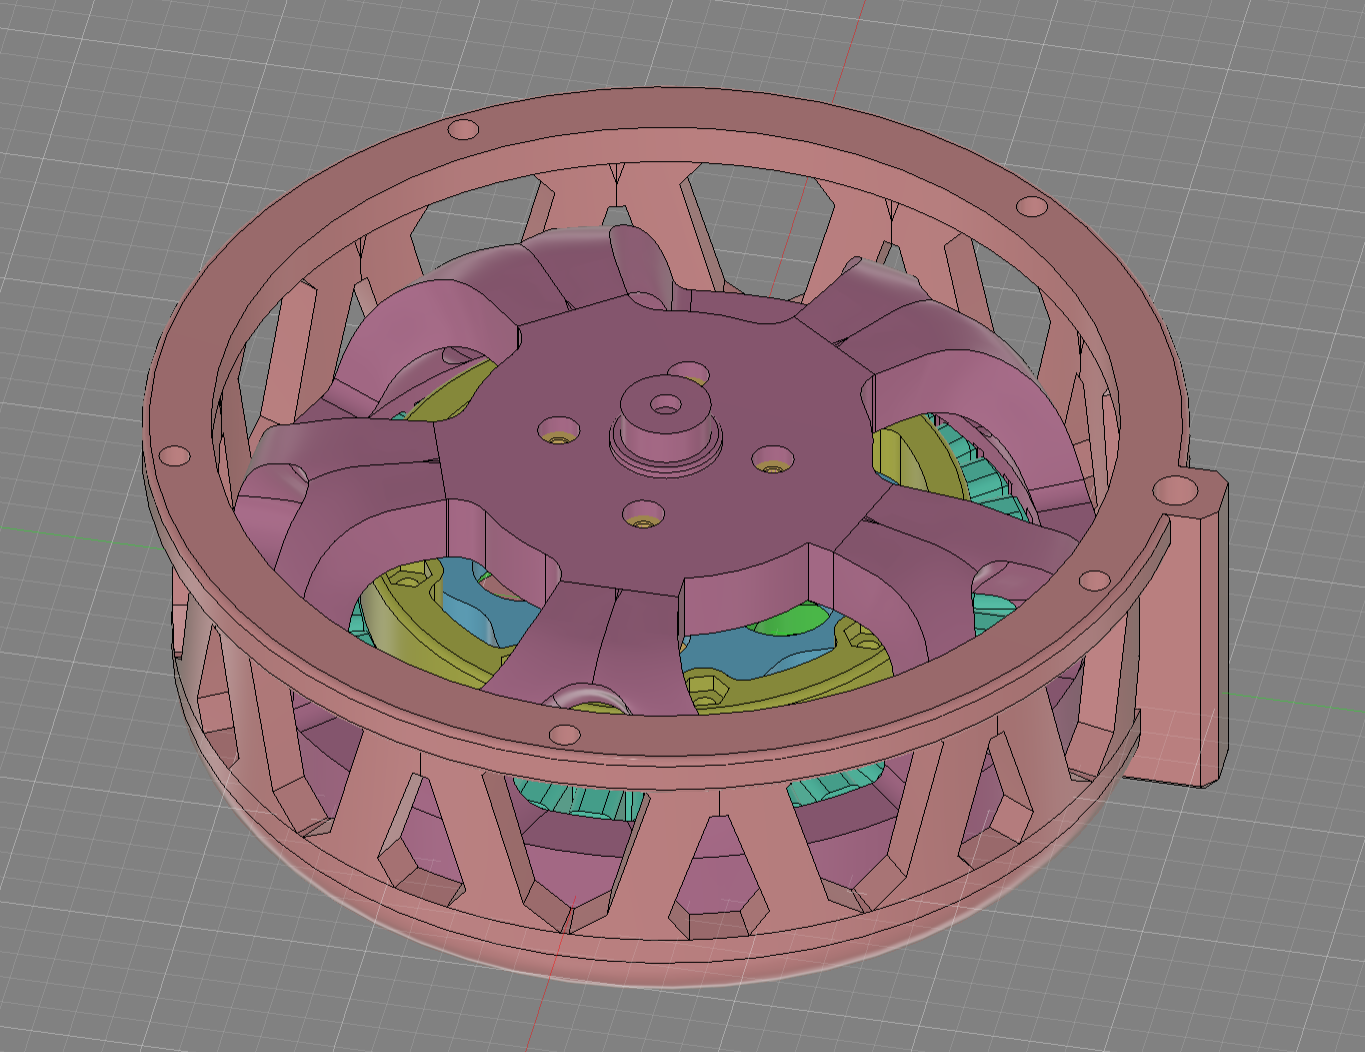
\includegraphics[width=\linewidth]{Images/Motor/InternalV1.png}
        \caption{Internal Cycloidal Drive First Version}
    \end{figure}
    \item The entire prototype was 3D printed in plastic and assembled with bearings and screws.
    \item Tests of motor and the cycloidal drive movement were made with this new design.
\end{itemize}
\paragraph[short]{Results}
\begin{itemize}
    \item The Internal Cycloidal Drive was operational.
    Video: Video: \attachfile{Images/Motor/IntCycV1.gif}
    \begin{figure}[H]
        \centering
        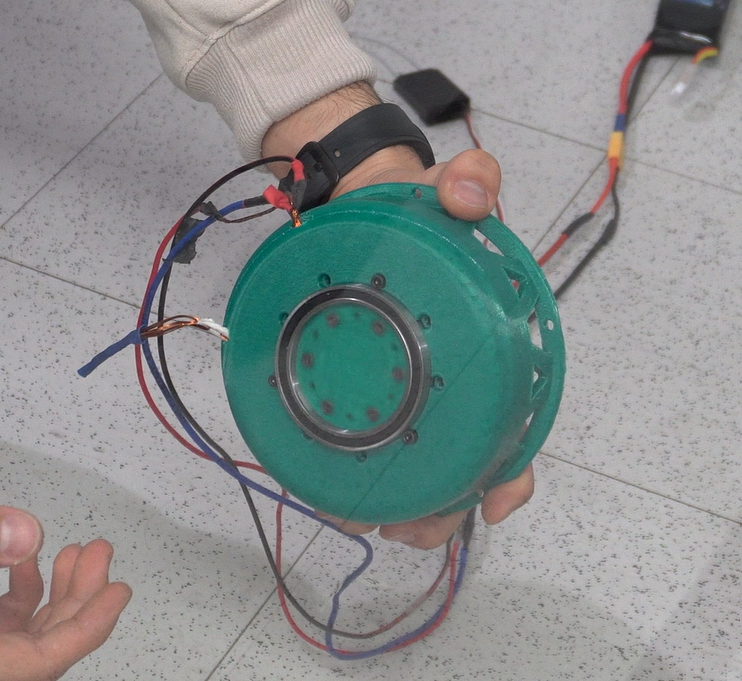
\includegraphics[width=\linewidth]{Images/Motor/IntCycV1Still.png}
        \caption{Internal Cycloidal Drive First Version}
    \end{figure}
    \item Some parts were too close together, causing friction and slightly hindering the motor's movement.
    \item The base lacked a component to prevent unwanted rotation of the cycloidal drive shaft, causing the motor to stop on some occasions.
\end{itemize}

\paragraph[short]{Conclusions}
\begin{itemize}
    \item Tolerances and the placement of some screws need to be corrected in the design to prevent collisions.
    \item A component should be implemented to keep the cycloidal drive shaft stable.
    \item Since the motor operates with its cycloidal drive, it is necessary to conduct speed and torque tests on the next prototype. Therefore, a test setup with the necessary sensors should be designed to obtain these data.
\end{itemize}

\subsubsection{Second \textbf{Internal} Cycloidal Drive prototype}
\paragraph[short]{Development}
\begin{itemize}
    \item A new prototype of the Internal Cycloidal Drive was designed, in which the screws on the output shaft holding the bearings were replaced with steel pins to support bushings, improving its stability. Additionally, sizes and distances between parts were corrected to prevent friction and reduce motor performance. A cover was also implemented on the base to stabilize the rotor and the cycloidal drive shaft.
    \item The entire prototype was 3D printed in plastic and assembled with bearings, bushings. steel pins and screws.
    
\end{itemize}
\paragraph[short]{Results}
\begin{itemize}
    \item The assembly was fully done, which is easier than the previous prototype
    \begin{figure}[H]
        \centering
        \begin{subfigure}{.5\textwidth}
          \centering
          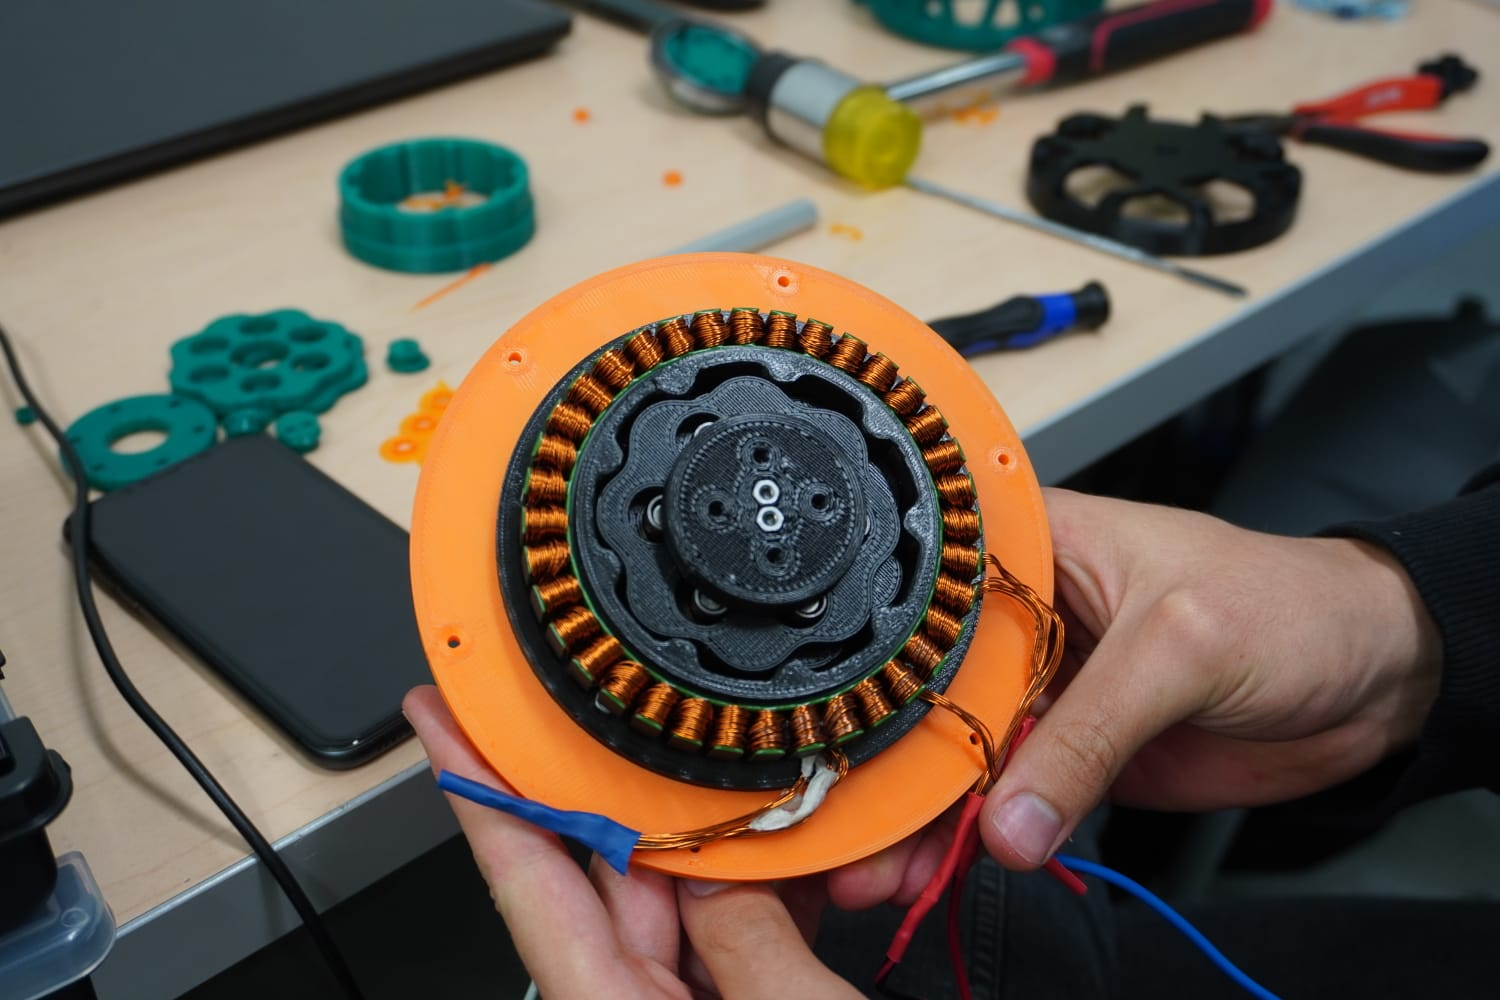
\includegraphics[width=.9\linewidth]{Images/Motor/IntCycV2A.jpg}
          \caption{Internal View}
          
        \end{subfigure}%
        \begin{subfigure}{.5\textwidth}
          \centering
          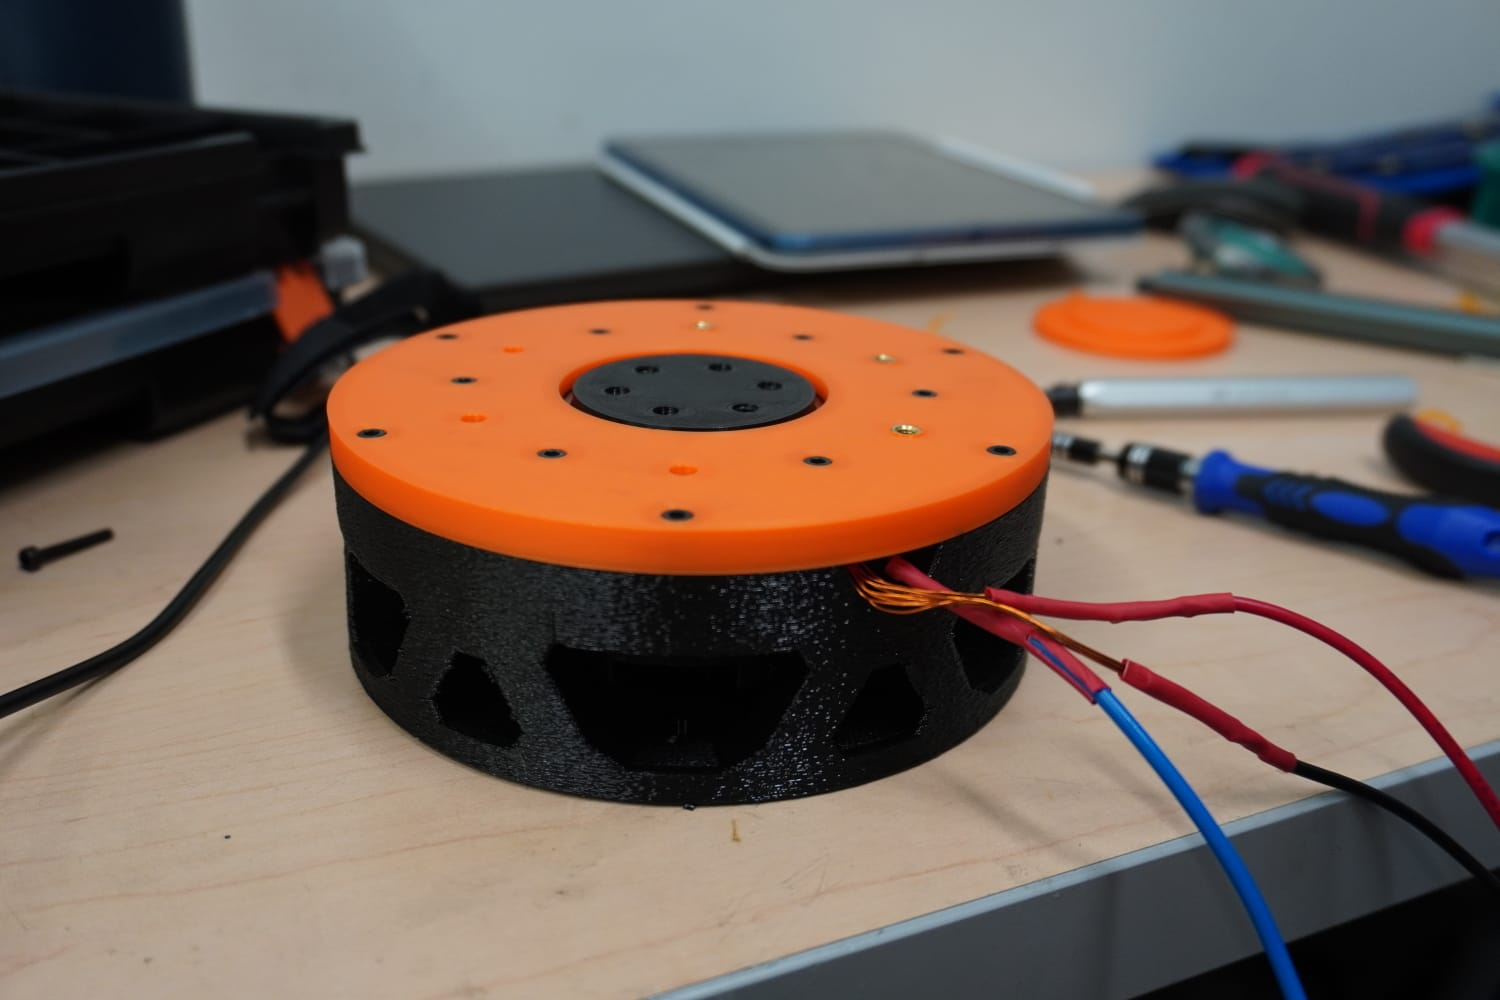
\includegraphics[width=.9\linewidth]{Images/Motor/IntCycV2B.jpg}
          \caption{Fll Assembly}
          
        \end{subfigure}
       
        \caption{Internal Cycloidal Drive - Second Prototype}
    \end{figure}
    \item The motor Spins correctly and its much more stable when spinning. 
    \textbf{Video: \attachfile{Images/Motor/IntCycV2.gif}}
    \begin{figure}[H]
        \centering
        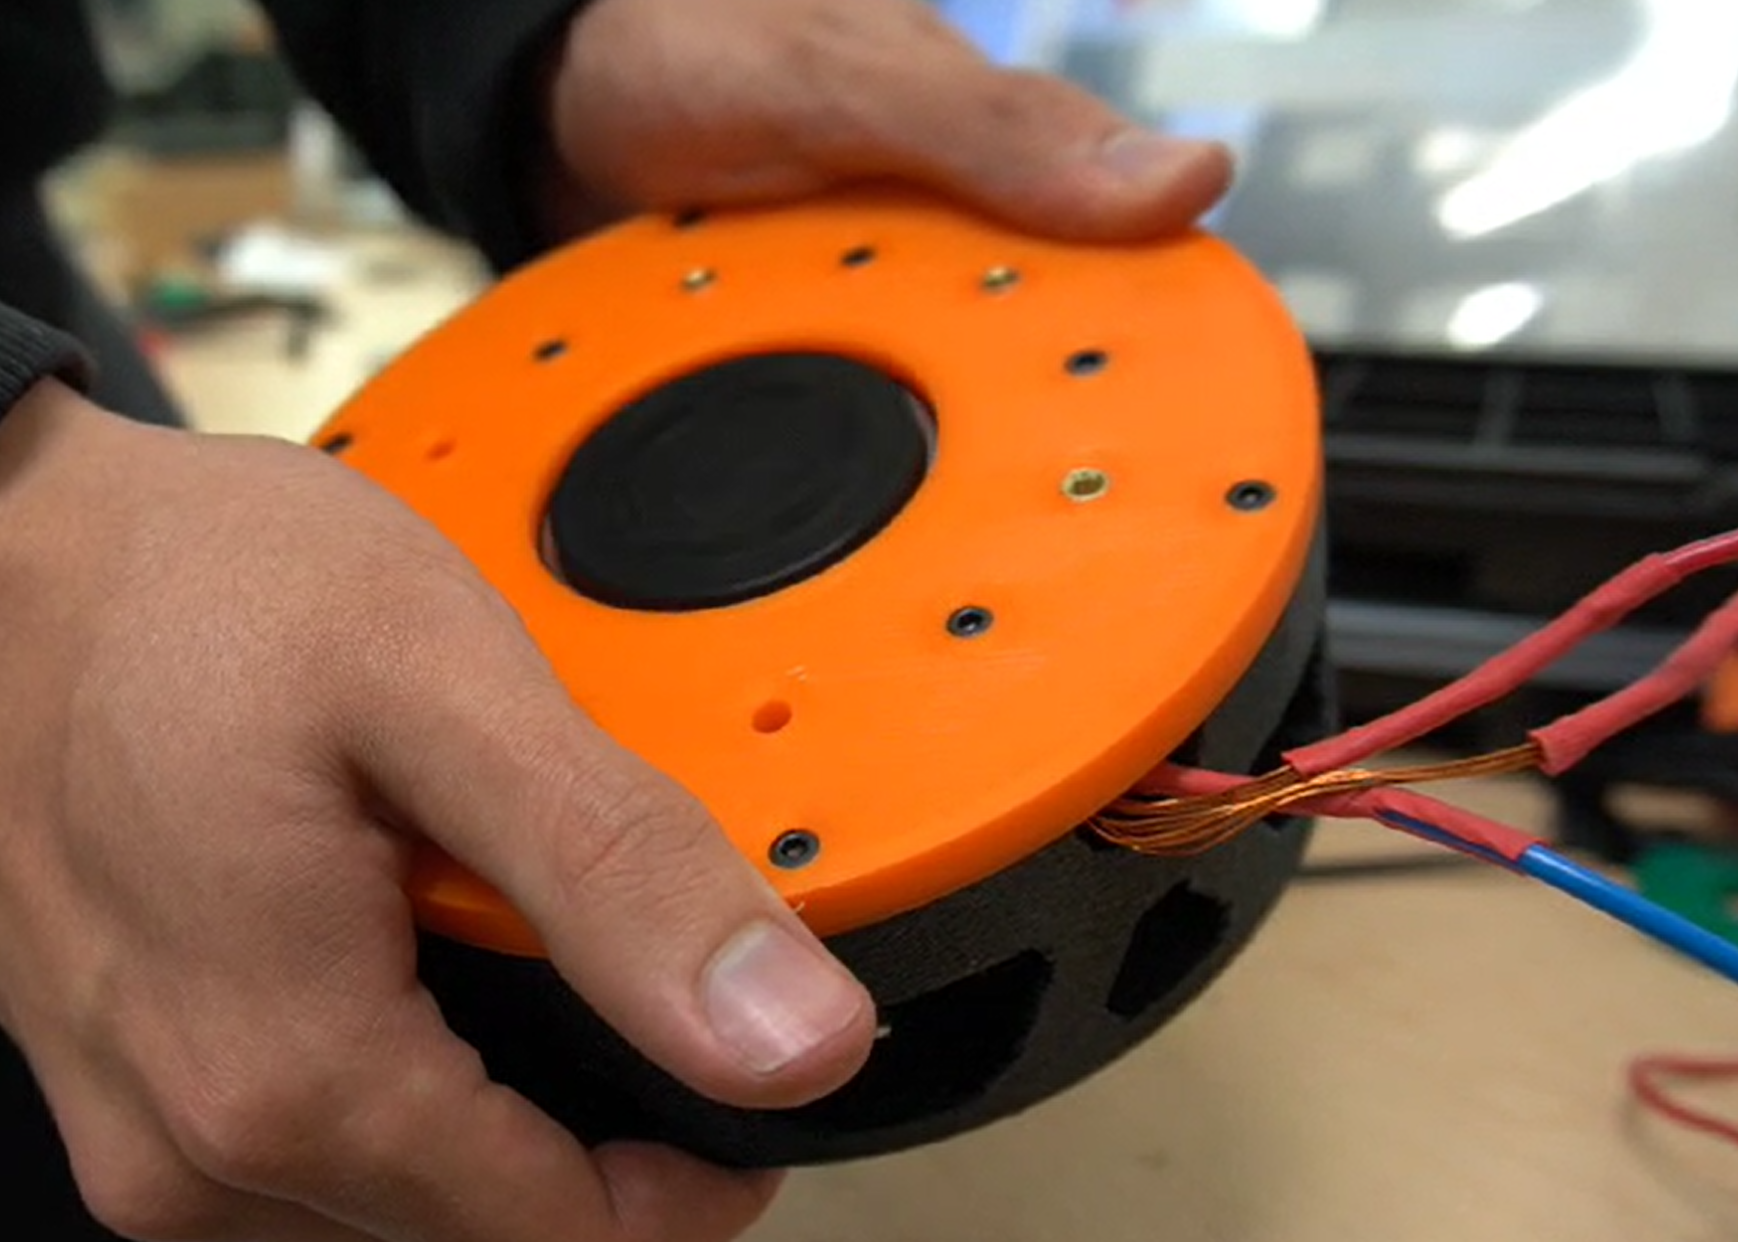
\includegraphics[width=\linewidth]{Images/Motor/IntCycV2Spin.png}
        \caption{Internal Cycloidal Drive Second Version}
    \end{figure}
\end{itemize}

\paragraph[short]{Conclusions}
\begin{itemize}
    \item It is neccessary to test the maximun torque of the motor
    \item A design made in more durable materials is neccessary for long term application, so CNC machining some pieces is needed to be explored
    \item There are some aspects about the design that need to be polished
\end{itemize}

\subsection{Chasis}
\subsubsection[]{First Prototype}
\paragraph{Development}
\begin{itemize}
    \item Qualitative analysis of the possible viable structures for the Rover's chassis
    \item CAD design of the desired chassis structure
    \item Material and component analysis of how the chassis will be
    \item Three alternatives were presented for the chassis model. The first was a traditional square design, which had advantages in terms of ease of assembly and manufacturing, a simple and stable design but not very innovative. On the other hand, an irregular octagon design posed a structural challenge in terms of weight and simplicity but was innovative, compact for the necessary components, and had personality. Finally, a race car design that was not developed because it was far too complex; it was more attractive than functional. 
    
\end{itemize}

\paragraph{Results}
\begin{itemize}
    \item Based on the analysis made according to the possible chassis designs we opted for the irregular octagon as it represented a balance of innovation and personality with manufacturability and stable structure.
    \item A CAD design of the base structure was developed with the appropriate measurements to contain all components in an orderly and clean manner.
    
    \begin{figure}[H]
        \centering
        \begin{subfigure}{.5\textwidth}
          \centering
          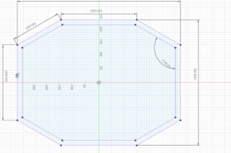
\includegraphics[width=.9\linewidth]{Images/Chasis/SketchV1.png}
          \caption{Chasis V1 - Sketch}
          
        \end{subfigure}%
        \begin{subfigure}{.5\textwidth}
          \centering
          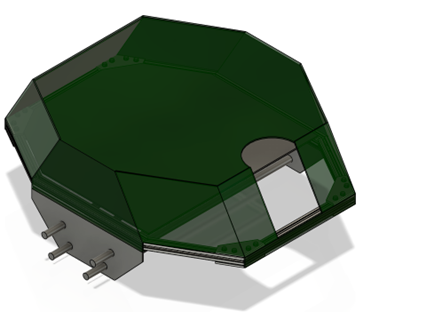
\includegraphics[width=.9\linewidth]{Images/Chasis/ChasisV1.png}
          \caption{Chasis V1 - 3D}
          
        \end{subfigure}
       
        \caption{Chasis concept}
    \end{figure}

    \item Various profiles and extrusions were reviewed, determining that 20x20 aluminum extrusions are versatile and offer ideal modularity for the Rover. However, the idea of using sheets is not discarded, as further research might allow manufacturing a chassis with good integrity and strength, depending on the design, sheet gauge, and support points. Manufacturable couplings were also created to assemble the Rover easily.
    \begin{figure}[H]
        \centering
        \begin{subfigure}{.3\textwidth}
          \centering
          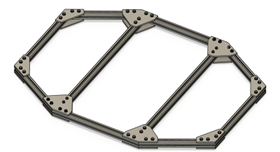
\includegraphics[width=.9\linewidth]{Images/Chasis/Extrusions1.png}

          
        \end{subfigure}%
        \begin{subfigure}{.3\textwidth}
          \centering
          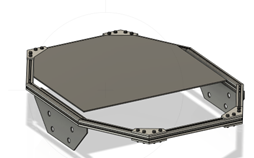
\includegraphics[width=.9\linewidth]{Images/Chasis/Extrusions2.png}

          
        \end{subfigure}
        \begin{subfigure}{.3\textwidth}
            \centering
            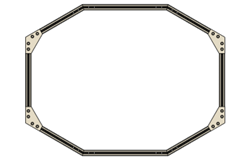
\includegraphics[width=.9\linewidth]{Images/Chasis/Extrusions3.png}
  
            
          \end{subfigure}
        \caption{Extrusions Assemblies}
        
    \end{figure}

    \item Based on the design and possible materials for these supports and couplings, 1020 steel was selected because its low carbon concentration allows for a softer and more ductile material, meaning it can be easily deformed without cracking, and 6061 aluminum, as these materials meet our needs for strength, durability, and lightness.
    \item The weight of the chassis, including screws and supports, is approximately 6 kg.
    \item The structure has a safety factor of 1.75, which means that the design will not fail but is open to improvements regarding the supports and load distribution. The image shows an adjusted deformation, but the actual deformation is 1.731mm, so it will not affect the integrity of the structure. Additionally, it can withstand up to 157.185 MPa, making it reliable.
    \begin{figure}[H]
        \centering
        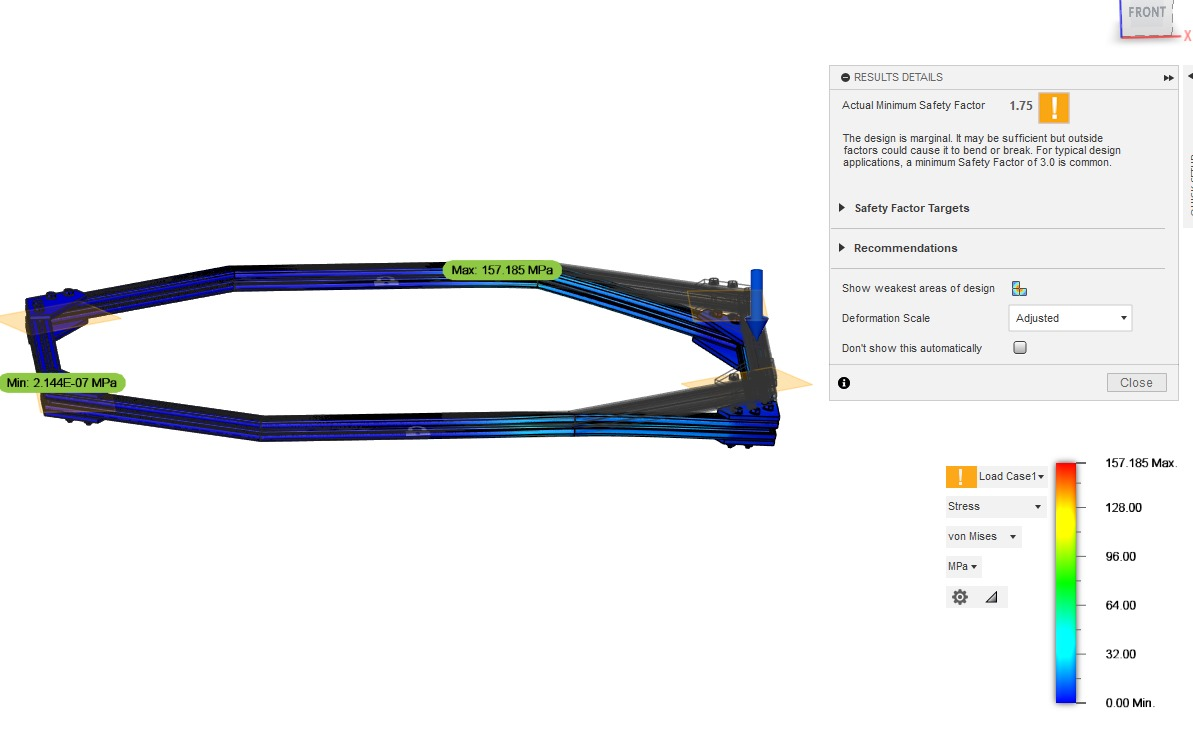
\includegraphics[width=\linewidth]{Images/Chasis/Sim1.jpg}
        \caption{Chasis Simulation}
    \end{figure}
\end{itemize}

\paragraph[short]{Conclusions}
\begin{itemize}
    \item The final geometry of the chassis is an irregular octagon due to its compactness, innovation, and personality. However, it is necessary to deepen the analysis of static and dynamic loads to ensure the success of the design.
    \item The use of 6061 aluminum and 1020 steel is ideal for the Rover’s applications and requirements.
    \item It is necessary to deepen the analysis of the support points with the rockers to finalize the chassis model and ensure a proper structure.
    \item An analysis of the arm with the Rover is required, since, despite being a stable structure, it is important to review the forces that the arm can generate when assembled in the Rover, as well as consider the weight of the parts it may lift.
    
\end{itemize}

\subsection{Rockers}

\subsubsection{First Prototype}
\paragraph[short]{Development}
\begin{itemize}
    \item Brainstorming, analysis, and generation of concepts for a stabilization system for the Rover.
    \item Preliminary CAD design of the selected geometry.
    \item Estimation of materials and manufacturing costs for the chosen design.
    \item Various options were presented and analyzed:
    \begin{figure}[H]
        \centering
        \begin{subfigure}{.3\textwidth}
          \centering
          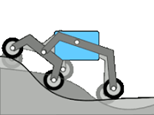
\includegraphics[width=.9\linewidth]{Images/Rockers/Concept1.png}
          \caption{First Concept}
          
        \end{subfigure}%
        \begin{subfigure}{.3\textwidth}
          \centering
          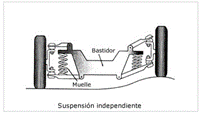
\includegraphics[width=.9\linewidth]{Images/Rockers/Concept2.png}
          \caption{Second Concept}
          
        \end{subfigure}
        \begin{subfigure}{.3\textwidth}
            \centering
            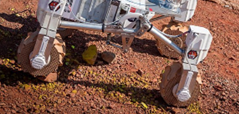
\includegraphics[width=.9\linewidth]{Images/Rockers/Concept3.png}
            \caption{Thrid Concept}
            
          \end{subfigure}
        \caption{Rockers Concepts}
        
    \end{figure}

\end{itemize}
\paragraph[short]{Results}
\begin{itemize}

    \item After evaluating factors such as reliability, weight, performance, cost, and adaptability to change, among others, an independent suspension system was selected. This system would significantly enhance the Rover's versatility in traversing uneven terrains and greatly improve its resistance to tipping over.
    \begin{figure}[H]
        \centering
        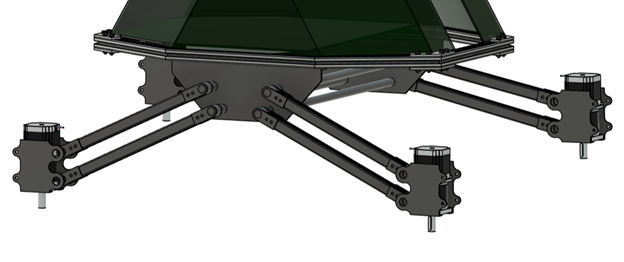
\includegraphics[width=\linewidth]{Images/Rockers/RockersV1.png}
        \caption{Rockers 3d Model with Chasis}
    \end{figure}
\end{itemize}



\paragraph[short]{Conclusions}
\begin{itemize}
    \item The final geometry of the rocker system implements a 4-bar parallel system, ensuring that the motors responsible for the vertical rotation of the wheels remain perpendicular to the ground.
    \item Aluminum extrusions and steel sheets will be used for constructing the structure.
    \item The axles will be built using copper and steel bushings.
    \item The selection of shock absorbers is pending, depending on the final geometry of the chassis and the weight distribution within it.
    \item Simulations and geometric adjustments will determine the final version of the system.
\end{itemize}


\subsection[]{Wheels}

\subsubsection{First Protoype}
\paragraph[short]{Development}
\begin{itemize}
    \item A tire prototype was created, consisting of a single piece of TPU (Thermoplastic Polyurethane) material.
    \item A support ring made of stainless steel was added to withstand the forces.
    \begin{figure}[H]
        \centering
        \begin{subfigure}{.5\textwidth}
          \centering
          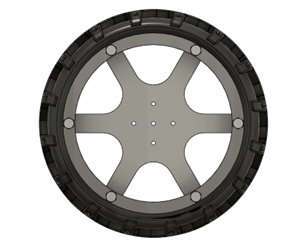
\includegraphics[width=.8\linewidth]{Images/Wheels/FrontViewP1.png}
          \caption{Front View}
          
        \end{subfigure}%
        \begin{subfigure}{.5\textwidth}
          \centering
          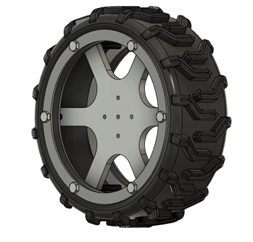
\includegraphics[width=.8\linewidth]{Images/Wheels/SideViewP1.png}
          \caption{Side View}
          
        \end{subfigure}
        \caption{First Wheel prototype - 3D}
        
        \end{figure}
    \item Simulations were conducted to determine the approximate weight of the assembly using TPU and stainless steel.
\end{itemize}
\paragraph[short]{Results}
\begin{itemize}
    \item Simulations showed that the complete tire assembly would weigh a little over 4 kg.
    \item This weight was significantly higher than planned, exceeding the weight limit of 2 kg.
    \item Various strategies were attempted to reduce the weight, including material removal and additional structural analyses.
\end{itemize}

\paragraph[short]{Conclusions}
\begin{itemize}
    \item The initial prototype was not viable as its weight exceeded the established limit.
    \item Despite efforts to reduce the weight, the desired goal was not achieved.
    \item Other design options and materials need to be explored to meet the weight requirements.
\end{itemize}

\subsubsection{Second Protoype}
\paragraph[short]{Development}
\begin{itemize}
    \item A 3D model of the rover's tire was designed, with static structural simulations conducted to evaluate its performance.
    The tire was divided into two parts:
    \begin{itemize}
        \item Internal Part (Ring): Made with PLA using 3D printing.
        \item External Part (Tread): A thin layer of TPU, also 3D printed.
    \end{itemize}
    
    \begin{figure}[H]
        \centering
        \begin{subfigure}{.5\textwidth}
          \centering
          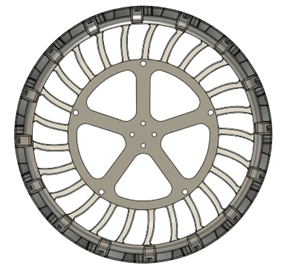
\includegraphics[width=.9\linewidth]{Images/Wheels/FrontViewP2.png}
          \caption{Front View}
          
        \end{subfigure}%
        \begin{subfigure}{.5\textwidth}
          \centering
          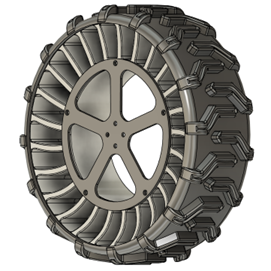
\includegraphics[width=.9\linewidth]{Images/Wheels/SideViewP2.png}
          \caption{Side View}
          
        \end{subfigure}
        \caption{Second Wheel prototype - 3D}
        
    \end{figure}
    
    \item Various shapes and structures of the ring were evaluated to ensure it could support the weight of the rover.
\end{itemize}
\paragraph[short]{Results}
\begin{itemize}
    \item Simulations indicated that the design would support the rover's weight while minimizing the total weight of the tire. \attachfile{Images/Wheels/SimP2.gif}
    \begin{figure}[H]
        \centering
        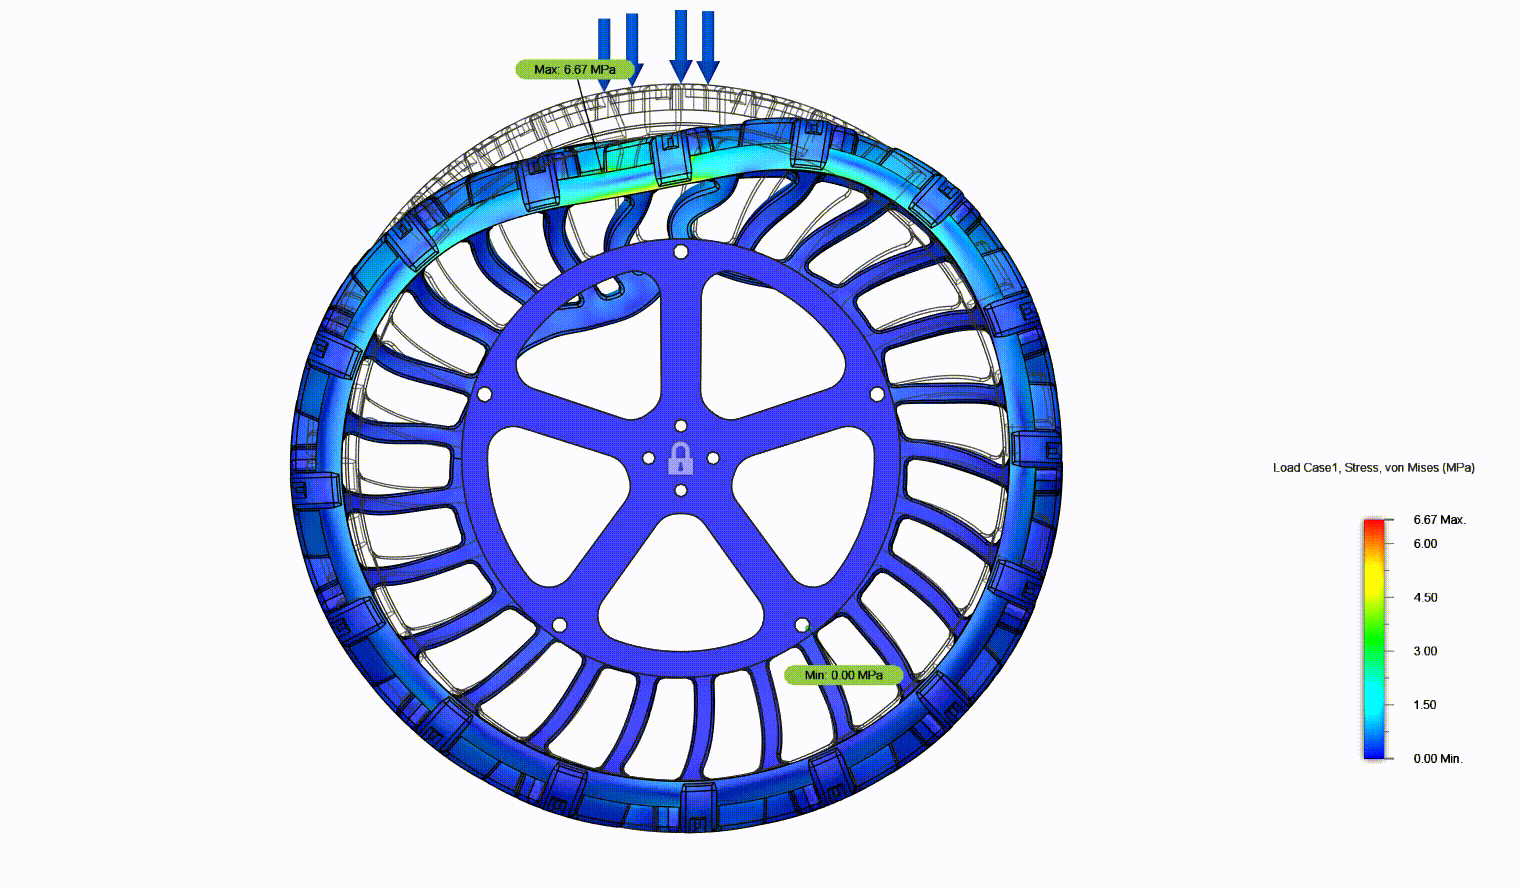
\includegraphics[width=\linewidth]{Images/Wheels/SimP2-10.png}
        \caption{Second Protoype Simulation - 50kg of pressure}
    \end{figure}
    \item The simulation gave a security factor of 15.
    \item The approximate weight of the tire, including all its parts, was estimated to be around 2 kg.
    \item The use of polymer resin was considered as an alternative to PLA and TPU to reduce production times.
\end{itemize}

\paragraph[short]{Conclusions}
\begin{itemize}
    \item The current tire design is structurally viable and meets the objective of minimizing weight.
    \item Manufacturing using 3D-printed PLA and TPU can be optimized by using polymer resin, which could significantly reduce production time.
    \item Reducing manufacturing times is crucial for the efficiency of the project, and this alternative is being actively investigated.
\end{itemize}



\subsection{Design and Brand}
\subsubsection{Defining Mision, Vision, Objectives and Values}
\paragraph{Development}
\begin{itemize}
    \item Investigated examples of robotics’ teams and companies for reference. Those references were rather visual or conceptual, which helped us to define our possible contribution in the robotic industry (local or global).
    \begin{figure}[H]
        \centering
        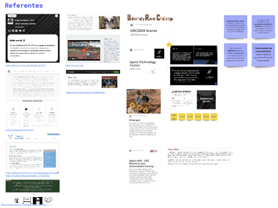
\includegraphics[width=\linewidth]{Images/Design/Miro1.png}
        \caption{Miro Board}
    \end{figure}
    \item Brainstormed with the team members keywords and phrases which we thought would describe our work. 
    
    \item Started writing paragraphs which connected the ideas from the brainstorm to create the mission, vision and objectives. 
    \begin{figure}[H]
        \centering
        \begin{subfigure}[b]{0.475\textwidth}
            \centering
            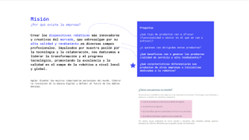
\includegraphics[width=\textwidth]{Images/Design/MisionV1.png}
            \caption[First version - Mision]%
            {{\small First version - Mision}}    
            
        \end{subfigure}
        \hfill
        \begin{subfigure}[b]{0.475\textwidth}  
            \centering 
            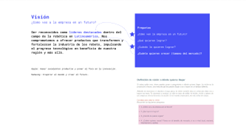
\includegraphics[width=\textwidth]{Images/Design/VisionV1.png}
            \caption[]%
            {{\small First version - Vision}}    
            
        \end{subfigure}
        \vskip\baselineskip
        \begin{subfigure}[b]{0.475\textwidth}   
            \centering 
            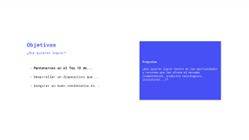
\includegraphics[width=\textwidth]{Images/Design/ObjetivosV1.png}
            \caption[]%
            {{\small First version - Objectives}}    
            
        \end{subfigure}
        \hfill
        \begin{subfigure}[b]{0.475\textwidth}   
            \centering 
            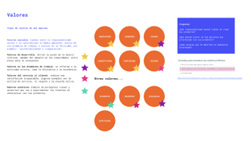
\includegraphics[width=\textwidth]{Images/Design/ValoresV1.png}
            \caption[]%
            {{\small First version - Values}}    
            
        \end{subfigure}
        
    \end{figure}
    \item Created mood boards according to the objectives and motivations of the team, representing sensations, collaborative goals and how consumers will perceive us as a team. 
    \begin{figure}[H]
        \centering
        \begin{subfigure}{.5\textwidth}
          \centering
          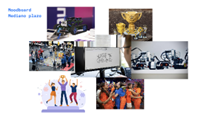
\includegraphics[width=.8\linewidth]{Images/Design/Moodboard1.png}
          \caption{Medium term Mood Board}
          
        \end{subfigure}%
        \begin{subfigure}{.5\textwidth}
          \centering
          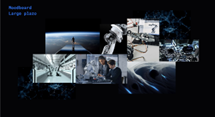
\includegraphics[width=.8\linewidth]{Images/Design/Moodboard2.png}
          \caption{Long Term Mood Board}
          
        \end{subfigure}
        \caption{Mood Boards}
        
    \end{figure}
\end{itemize}

\paragraph{Results}
\begin{itemize}
    \item A first version of the items was written and reviewed as a group. 
    \item Important ideas were highlighted and kept for a final version. During the discussion, we decided to be more specific and innovative regarding our contribution in the robotic industry,
    \item A second brainstorming session was held, with more specific guiding questions to finalize details.
    \item A second and final version of the items was written.
    
    \begin{figure}[H]
        \centering
        \begin{subfigure}[b]{0.475\textwidth}
            \centering
            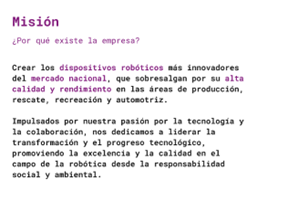
\includegraphics[width=\textwidth]{Images/Design/MisionV2.png}
            \caption[Second version - Mision]%
            {{\small Second version - Mision}}    
            
        \end{subfigure}
        \hfill
        \begin{subfigure}[b]{0.475\textwidth}  
            \centering 
            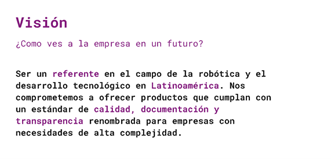
\includegraphics[width=\textwidth]{Images/Design/VisionV2.png}
            \caption[]%
            {{\small Second version - Vision}}    
            
        \end{subfigure}
        \vskip\baselineskip
        \begin{subfigure}[b]{0.475\textwidth}   
            \centering 
            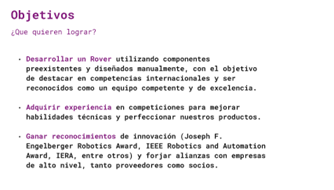
\includegraphics[width=\textwidth]{Images/Design/ObjetivosV2.png}
            \caption[]%
            {{\small Second version - Objectives}}    
            
        \end{subfigure}
        \hfill
        \begin{subfigure}[b]{0.475\textwidth}   
            \centering 
            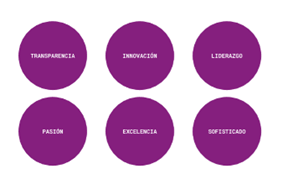
\includegraphics[width=\textwidth]{Images/Design/ValoresV2.png}
            \caption[]%
            {{\small Second version - Values}}    
            
        \end{subfigure}
        
    \end{figure}
    
\end{itemize}


\paragraph{Conclusions}
\begin{itemize}
    \item The group was excited to see their ideas and desires captured in clear words.
    \item We want to stand out through our quality and high performance, by developing components from scratch and having social and environmental responsibility.
    \item We describe ourselves as an innovative, passionate, sophisticated (among other values) team. 
    \item Clear goals were set.
    
\end{itemize}

\subsubsection{Defining Name, Color Palette and Fonts}
\paragraph{Development}
\begin{itemize}
    \item Within the design team, a first brainstorm was performed, in which each member suggested at least one name, color palette and title and text font. 
    \item Out of the first brainstorm, the design team selected their preferred options to show to the rest of the team. 
    \item Among the team, the favorites were voted. Suggestions were made, and a second brainstorm was performed to reselect color palette and fonts. 
    \item The new ideas were presented in a meeting. The color palette was built between all the team members. 
    \begin{figure}[H]
        \centering
        \begin{subfigure}{.5\textwidth}
          \centering
          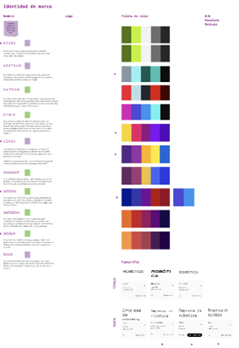
\includegraphics[width=.8\linewidth]{Images/Design/ColorsV1.png}
          \caption{Color Palette Proposal}
          
        \end{subfigure}%
        \begin{subfigure}{.5\textwidth}
          \centering
          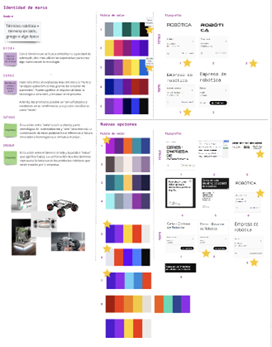
\includegraphics[width=.8\linewidth]{Images/Design/ColorsV2.png}
          \caption{Side View}
          
        \end{subfigure}
        \caption{Color Palette Development}
        
    \end{figure}

\end{itemize}

\paragraph{Results}
\begin{itemize}
    \item The name of team was chosen. 
    \item The color palette was chosen. 
    \begin{figure}[H]
        \centering
        \begin{subfigure}{.5\textwidth}
          \centering
          
\includegraphics[width=.8\linewidth]{Images/Design/Name.png}
          \caption{Name}
          
        \end{subfigure}%
        \begin{subfigure}{.5\textwidth}
          \centering
          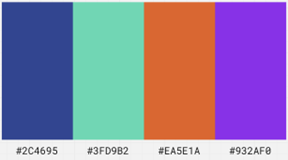
\includegraphics[width=.8\linewidth]{Images/Design/PaletteV1.png}
          \caption{Color Palette}
          
        \end{subfigure}
        \caption{Name and Color Palette}
        
    \end{figure}
    \item The title and text fonts were chosen. 
    \begin{figure}[H]
        \centering
        \begin{subfigure}{.5\textwidth}
          \centering
          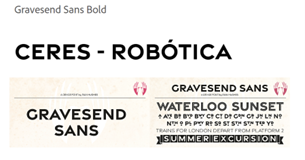
\includegraphics[width=.8\linewidth]{Images/Design/Font1V1.png}
          \caption{Title Font}
          
        \end{subfigure}%
        \begin{subfigure}{.5\textwidth}
          \centering
          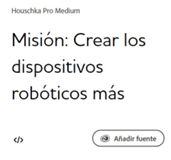
\includegraphics[width=.8\linewidth]{Images/Design/Font2V1.png}
          \caption{Normal Text Font}
          
        \end{subfigure}
        \caption{Fonts}
        
    \end{figure}

\end{itemize}


\paragraph{Conclusions}
\begin{itemize}
    \item The team was able to come to an agreement on the first items of the brand identity.
    \item The team agreed to develop a novel brand identity that confronts the usual robotic scheme, using bold colors and a light typography to connect with customers in an innovative way.
    \item The team was happy and excited to have an official name, color palette and fonts for representation. 
    
\end{itemize}

\subsubsection{Budget Panel}
\paragraph{Development}
\begin{itemize}
    \item We watched a tutorial to learn how to turn tables of data in Microsoft Excel into an interactive dashboard. 
    \item We drafted an idea of how the data will be distributed, emphasizing in the information that is more relevant for us and for potential sponsors.
    \item We made the interactive board with the purpose of making complex data legible for external parties, using mostly graphs and conventions.
    \begin{figure}[H]
        \centering
        \begin{subfigure}{.5\textwidth}
          \centering
          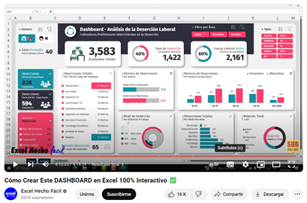
\includegraphics[width=.8\linewidth]{Images/Design/TutorialDash.png}
          \caption{Reference}
          
        \end{subfigure}%
        \begin{subfigure}{.5\textwidth}
          \centering
          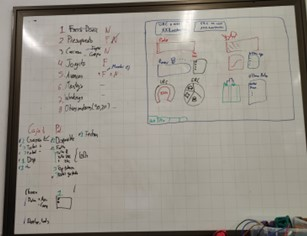
\includegraphics[width=.8\linewidth]{Images/Design/IdeaDash.jpg}
          \caption{DashBoard Brainstorm}
          
        \end{subfigure}
        \caption{Dashboard creative Process}
        
    \end{figure}
\end{itemize}


\paragraph{Results}
\begin{itemize}
    \item The dashboard was organized and properly linked to the data, using buttons and formulas to display different information.
    \item Several graphs were shown (lineal graph and ring graphs)
    \item The color palette previously selected was properly used. 
    \begin{figure}[H]
        \centering
        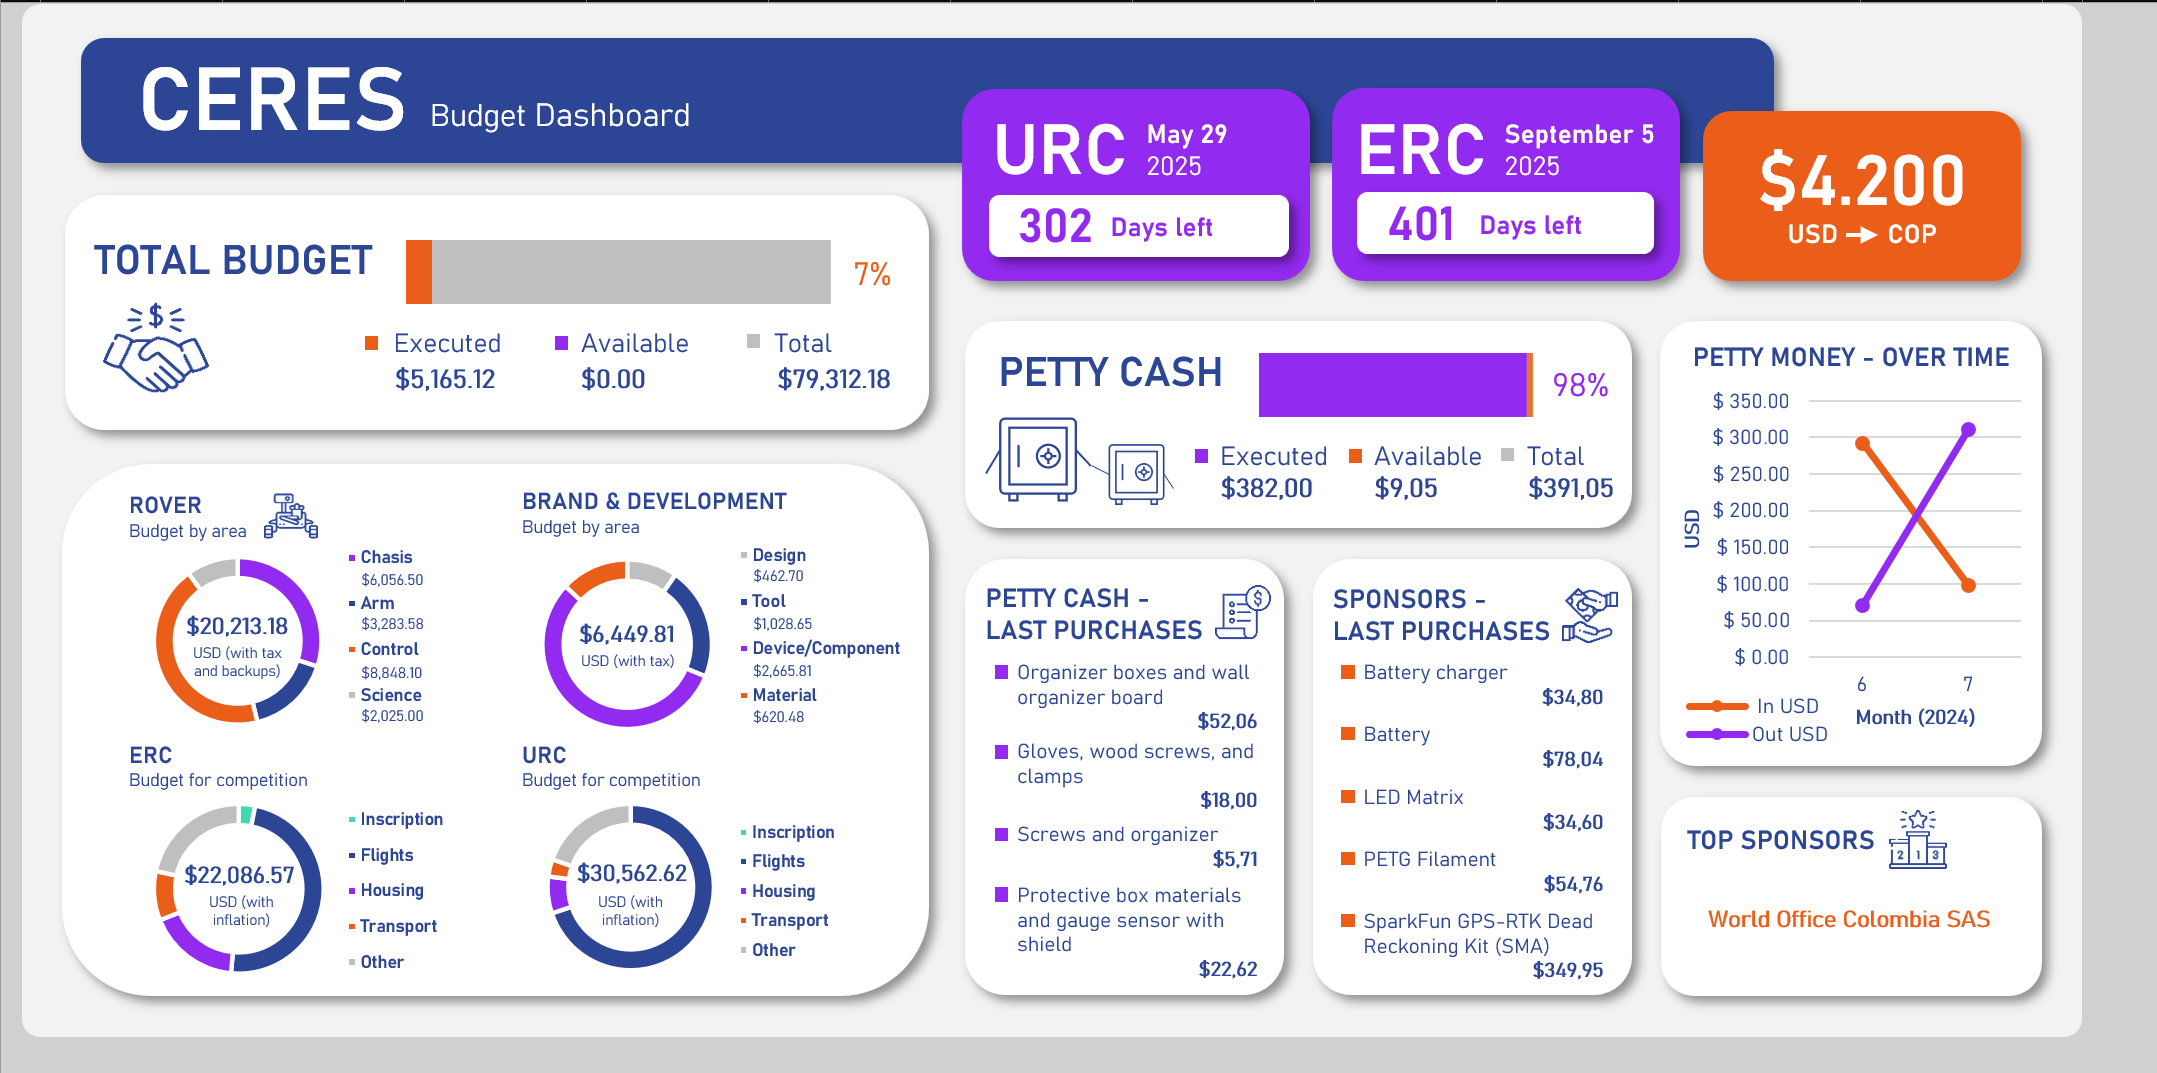
\includegraphics[width=\linewidth]{Images/Design/DashBoardV1.png}
        \caption{Dashboard}
    \end{figure}
\end{itemize}


\paragraph{Conclusions}
\begin{itemize}
    \item The dashboard was done to show the team and sponsor candidates all the resources and data in an organized and clear way.
    \item The interactive tools, such as buttons and formulas, makes the information more precise and legible for the viewers.
    \item The information hierarchies work effectively, making it clear to the viewer which data is most relevant within what the dashboard presents.
    
\end{itemize}



\subsection{Screen}
\paragraph[short]{Development}
\begin{itemize}
    \item Characterization of the LED matrix (64*32)
    \item Connection with Raspberry Pi Zero 2W
    \item Exploration of available libraries for its manipulation
\end{itemize}



\paragraph[short]{Results}
\begin{itemize}
    \item Visualization of test commands where it was possible to see the lighting and dimming of all the LEDs in the matrix as well as their color changes.
    \item Display of text input.
    \item Display of images, videos and .gif files.
    
    \textbf{Video: \attachfile{Images/Screen/gifScreen.mp4}}

    \begin{figure}[H]
        \centering
        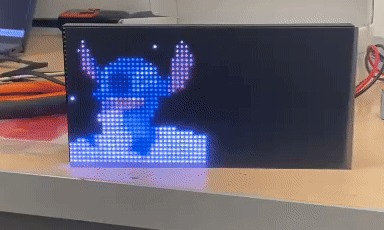
\includegraphics[width=\linewidth]{Images/Screen/Screen1.jpg}
        \caption{Video Display in Screen}
    \end{figure}
\end{itemize}

\paragraph[short]{Conclusion}
\begin{itemize}
    \item The LED matrix is easy to operate.
    \item Various visual elements can be displayed automatically by generating a folder of files stored within the controller.
    \item To achieve appropriate visualization, it is important to consider the dimensions of the input files relative to the matrix.
    \item To run a video file on the matrix, it will be necessary to implement a controller with greater capacity.
\end{itemize}

\section{Future Goals and Objectives}
The Following steps that are the most important for the development of the project are the following
\begin{itemize}
    \item Winding of the 4 motors of the wheels
    \item Test the control devices that arrived
    \begin{figure}[H]
        \centering
        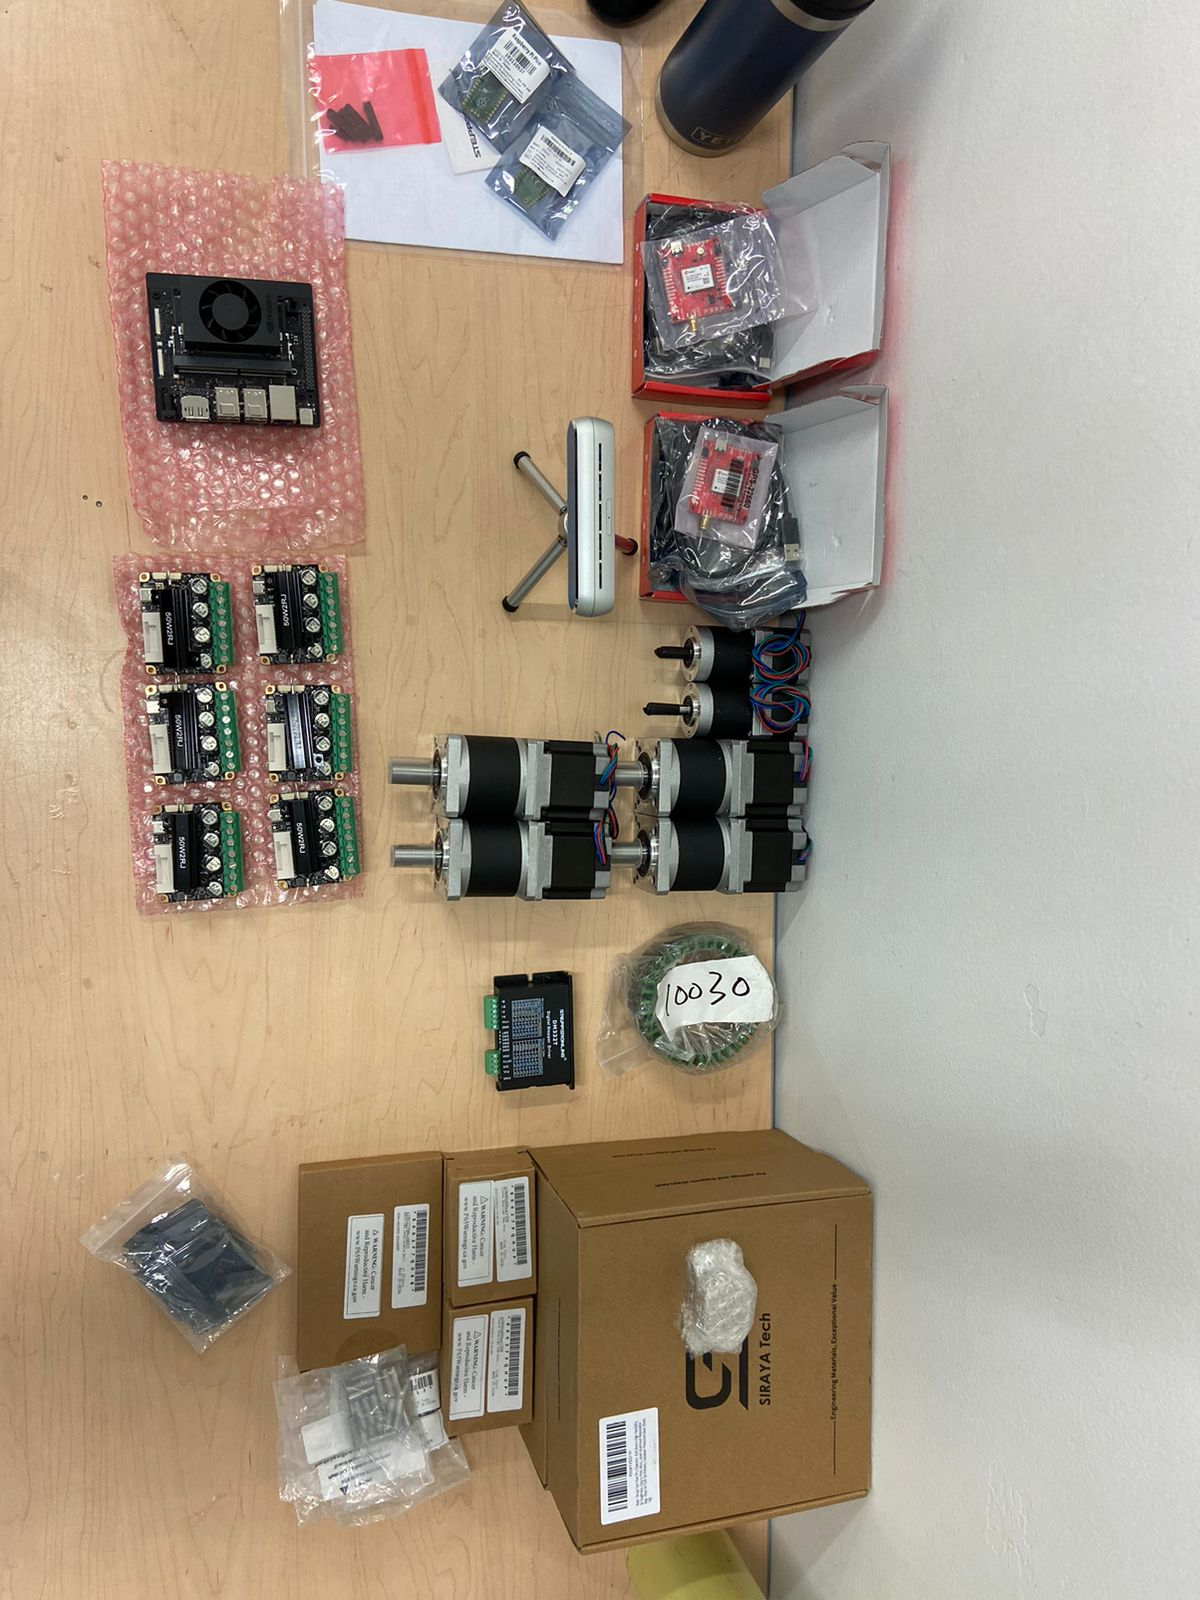
\includegraphics[width=\linewidth]{Images/Extra/PrimeraCompra.jpg}
        \caption{First Sponsor Items}
    \end{figure}
    \item Do a full characterization of the motor
    \item Finish the Chasis and Rockers desing to start the first assembly in Wood
    \item Continue simulation and brainstorming for the wheels
    \item Develop and select a Logo
    \item Start brainstorming the design od the arm
\end{itemize}

\end{document}
